An inverter with input $A$ and output $Q$ follows the following truth table:

\FloatBarrier

\begin{table}[h!]
	\centering
	\caption{Inverter Truth Table}
	\label{tab:inverter_tt}
	\csvautotabular{./tables/inverter_tt.csv}
\end{table}

\FloatBarrier

The inverter can then be realized in CMOS technology.
The width-to-length ratio of the inverter's NMOS shall be referred to as $n$ and $p$ for the PMOS.

\FloatBarrier

\begin{figure}[h!]
	\centering
	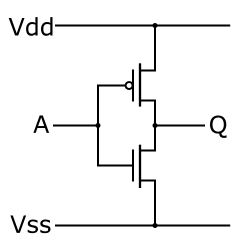
\includegraphics[scale=0.75]{./images/CMOS_Inverter.PNG}
	\caption{CMOS Inverter}
	\label{fig:CMOS_Inverter}
\end{figure}

\FloatBarrier

{\footnotesize Taken from link \url{https://en.wikipedia.org/wiki/CMOS#/media/File:CMOS_Inverter.svg}}

\FloatBarrier

A NAND gate with inputs $A$ and $B$ and output $C$ has a truth table given by:

\FloatBarrier

\begin{table}[h!]
	\centering
	\caption{NAND Truth Table}
	\label{tab:nand_tt}
	\csvautotabular{./tables/nand_tt.csv}
\end{table}

\FloatBarrier

The NAND gate can be implemented in CMOS like so:

\FloatBarrier

\begin{figure}[h!]
	\centering
	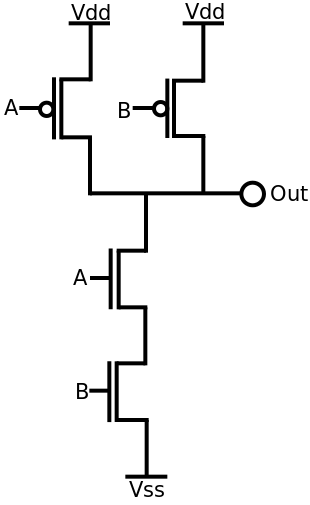
\includegraphics[scale=0.75]{./images/CMOS_NAND.PNG}
	\caption{CMOS NAND Gate}
	\label{fig:CMOS_NAND}
\end{figure}

\FloatBarrier

{\footnotesize Taken from link \url{https://upload.wikimedia.org/wikipedia/commons/e/e2/CMOS_NAND.svg}}

\FloatBarrier

Here, the width-to-length ratio of the NMOSs is $2n$ to compensate for the fact that the current driven from ground is halved in this series configuration.
The width-to-length ratio of the PMOSs is still $p$ since this issue does not occur with the parallel PMOSs.

The D-latch circuit is built using a CMOS inverter and four NAND gates, using two PMOS and two NMOS transistors each. The gate-level design is given in the figure below:

\FloatBarrier

\begin{figure}[h!]
	\centering
	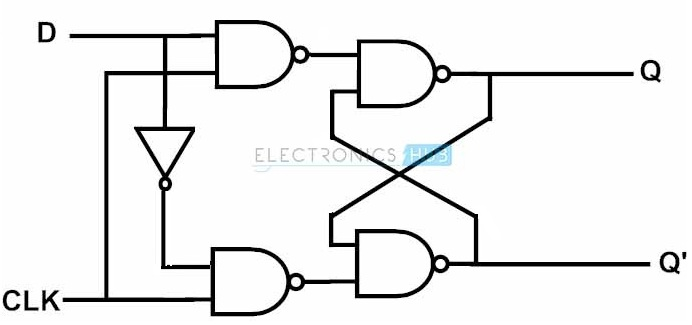
\includegraphics[scale=0.75]{./images/dlatchgates.PNG}
	\caption{D-Latch Gate Level Schematic}
	\label{fig:dlatchgates}
\end{figure}

\FloatBarrier

{\footnotesize Taken from link \url{https://www.electronicshub.org/d-flip-flop/}}

\FloatBarrier

The circuit is shown in figure (\ref{fig:spicecircuit}).

\FloatBarrier

\begin{figure}[h!]
	\centering
	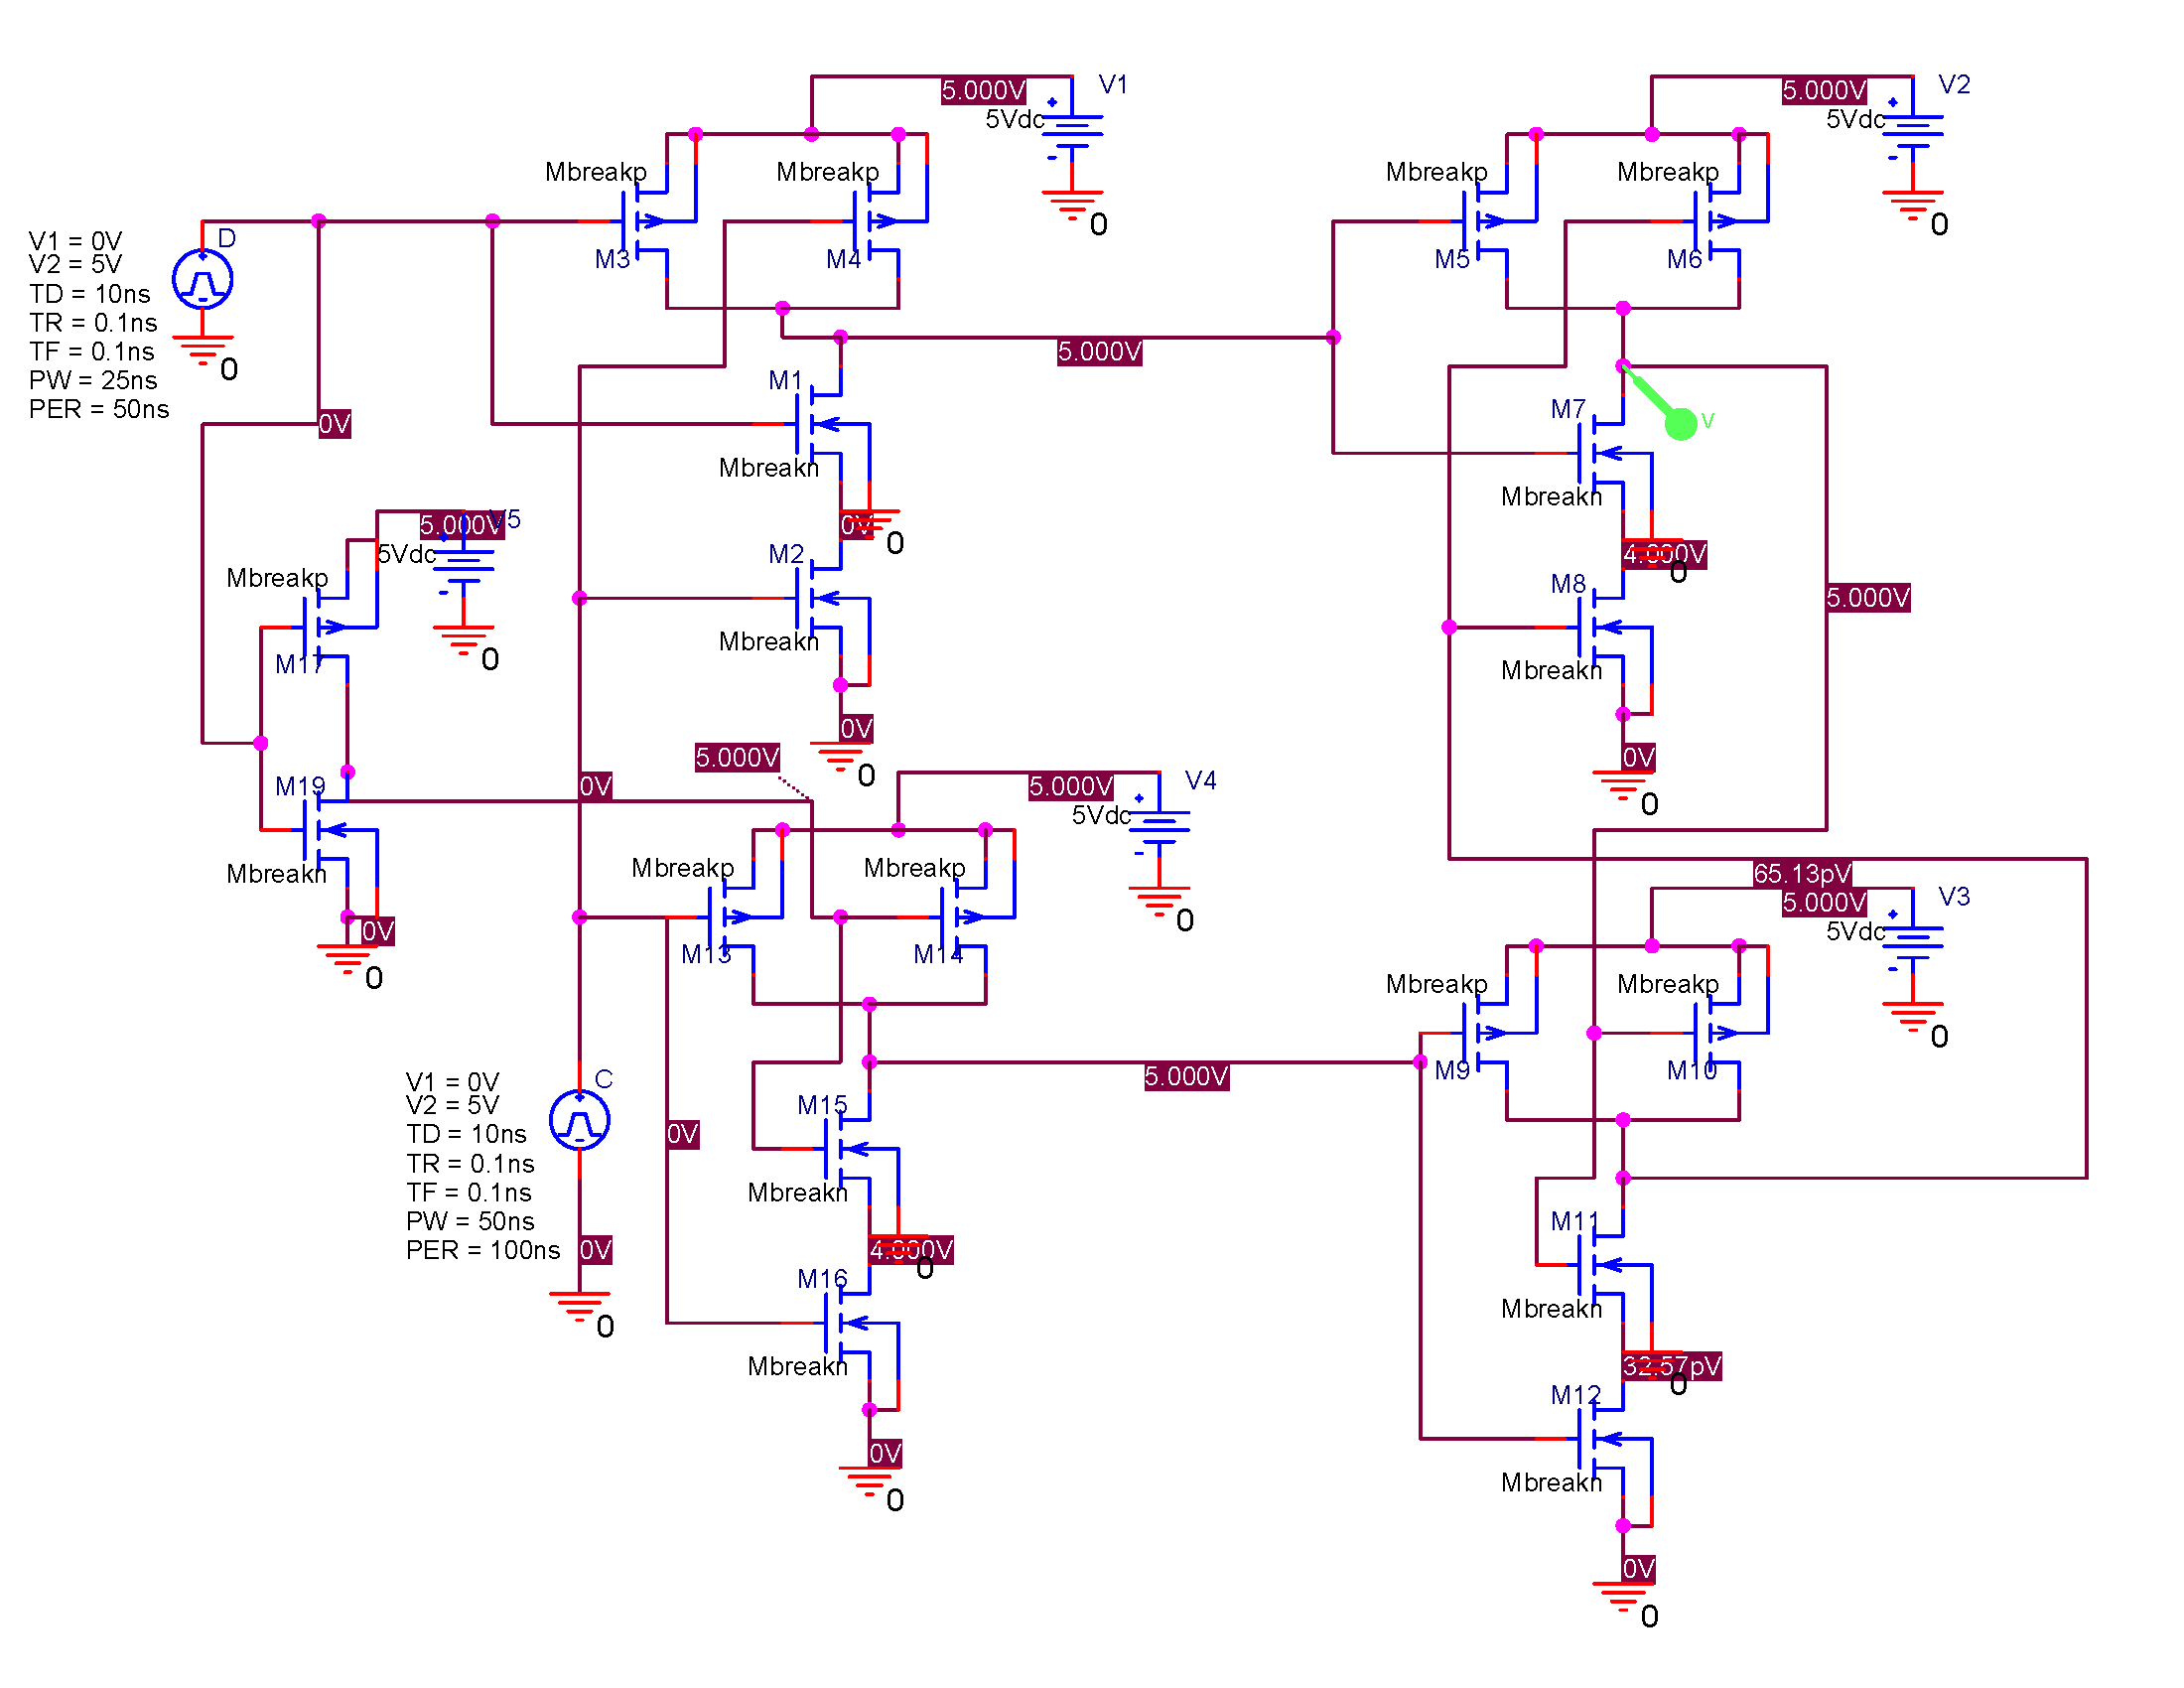
\includegraphics[width=1\linewidth]{./images/spice_circuit}
	\caption{The D-Latch Circuit Model for PSpice Simulation}
	\label{fig:spicecircuit}
\end{figure}

\FloatBarrier

When the control input, $C$, is high, the value of the input, $D$, is stored as the output value. However, when the control input is low, the value of the output cannot be changed. For example, if $D$ is high and $C$ high, the output $Q$ is high, but if $C$ is set to low, then the value of $D$ before the change is stored as the output value $Q$ until $C$ is brought high again. The behavior of the D-Latch is shown in the FSM in figure (\ref{fig:dlatch_fsm}).

The results of all the simulations are consistent with the assumed behavior of the D-Latch circuit. In figure (\ref{fig:spec_sim}), it is shown that when the control input $C$ is high the value of input $D$ is stored at the output $Q$, and when the control input $C$ is low the value of $D$ is not passed to the output $Q$. For this simulation, the settings in figure (\ref{fig:supplys}) are used for the inputs. These values are supplied in the lab specification document.

There is a small spike that occurs when $D$ is becoming high while $C$ is becoming low.
When this switch occurs, the bottom NAND gate of the SR latch portion of the design has one of its inputs change from $0$ to $1$.
The NAND gate includes two NMOSs in series.
When both inputs are $0$, the NMOSs act as open circuits, which are similar to two capacitors in series at DC.
When one of the inputs goes to $1$, one of the NMOSs turns on.
For a brief period of time, only one of the NMOSs is now an open circuit, whereas the other allows current to flow.
Assuming both NMOSs have the same effective "capacitance" when they are both off, the effective "capacitance" of the open circuit in the pull-down network doubles.
So, for a brief instant, current is drawn from supply and from the load capacitance connected to the output of the NAND gate.
This briefly pulls down the NAND gate's output, which is enough to send a brief $0$ pulse to the top latch, briefly setting $Q$ to $1$.
These effects quickly die out as the other NMOS becomes fully charged and acts as a pure open circuit again.
The values then return to the expected behavior.
However, this hypothesis is difficult to determine without further experimentation.

\FloatBarrier

\begin{figure}[h!]
	\centering
	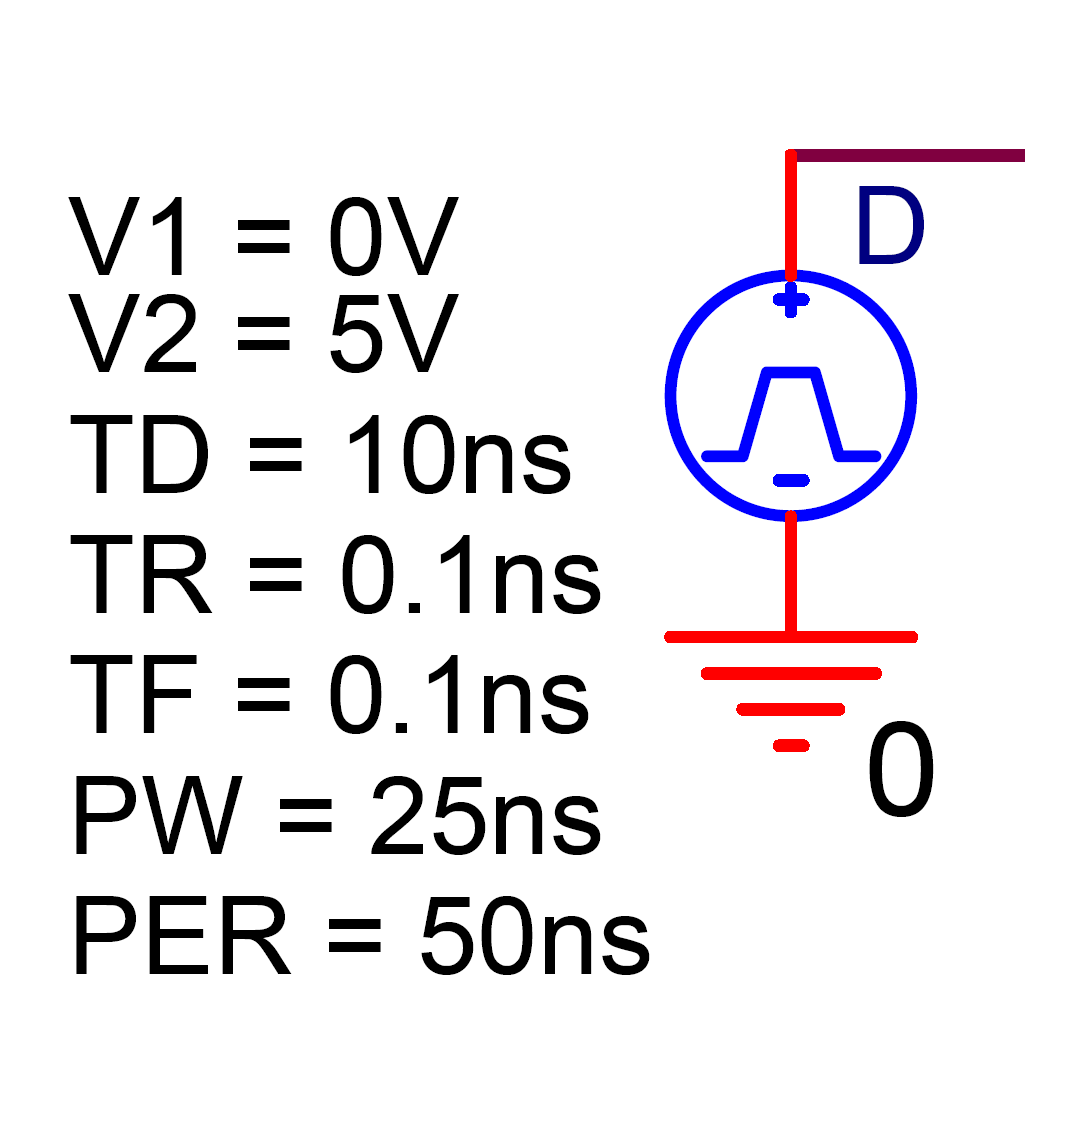
\includegraphics[width=0.4\textwidth]{./images/D_supply}
	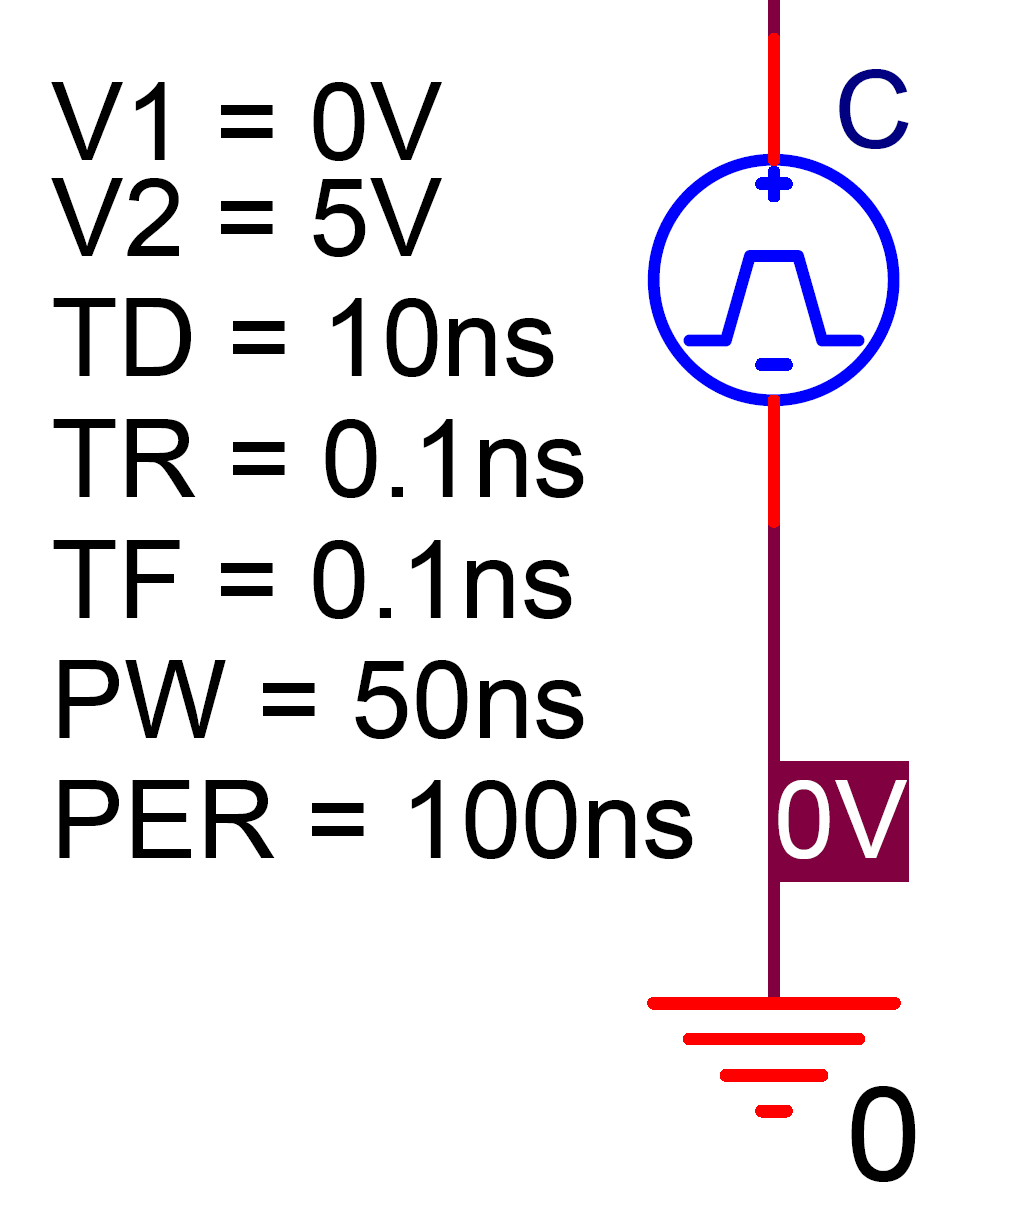
\includegraphics[width=0.4\textwidth]{./images/C_supply}
	\caption{The Simulated Input (Left) and the Simulated Control Input}
	\label{fig:supplys}
\end{figure}

\FloatBarrier

\FloatBarrier

\begin{figure}[h!]
	\centering
	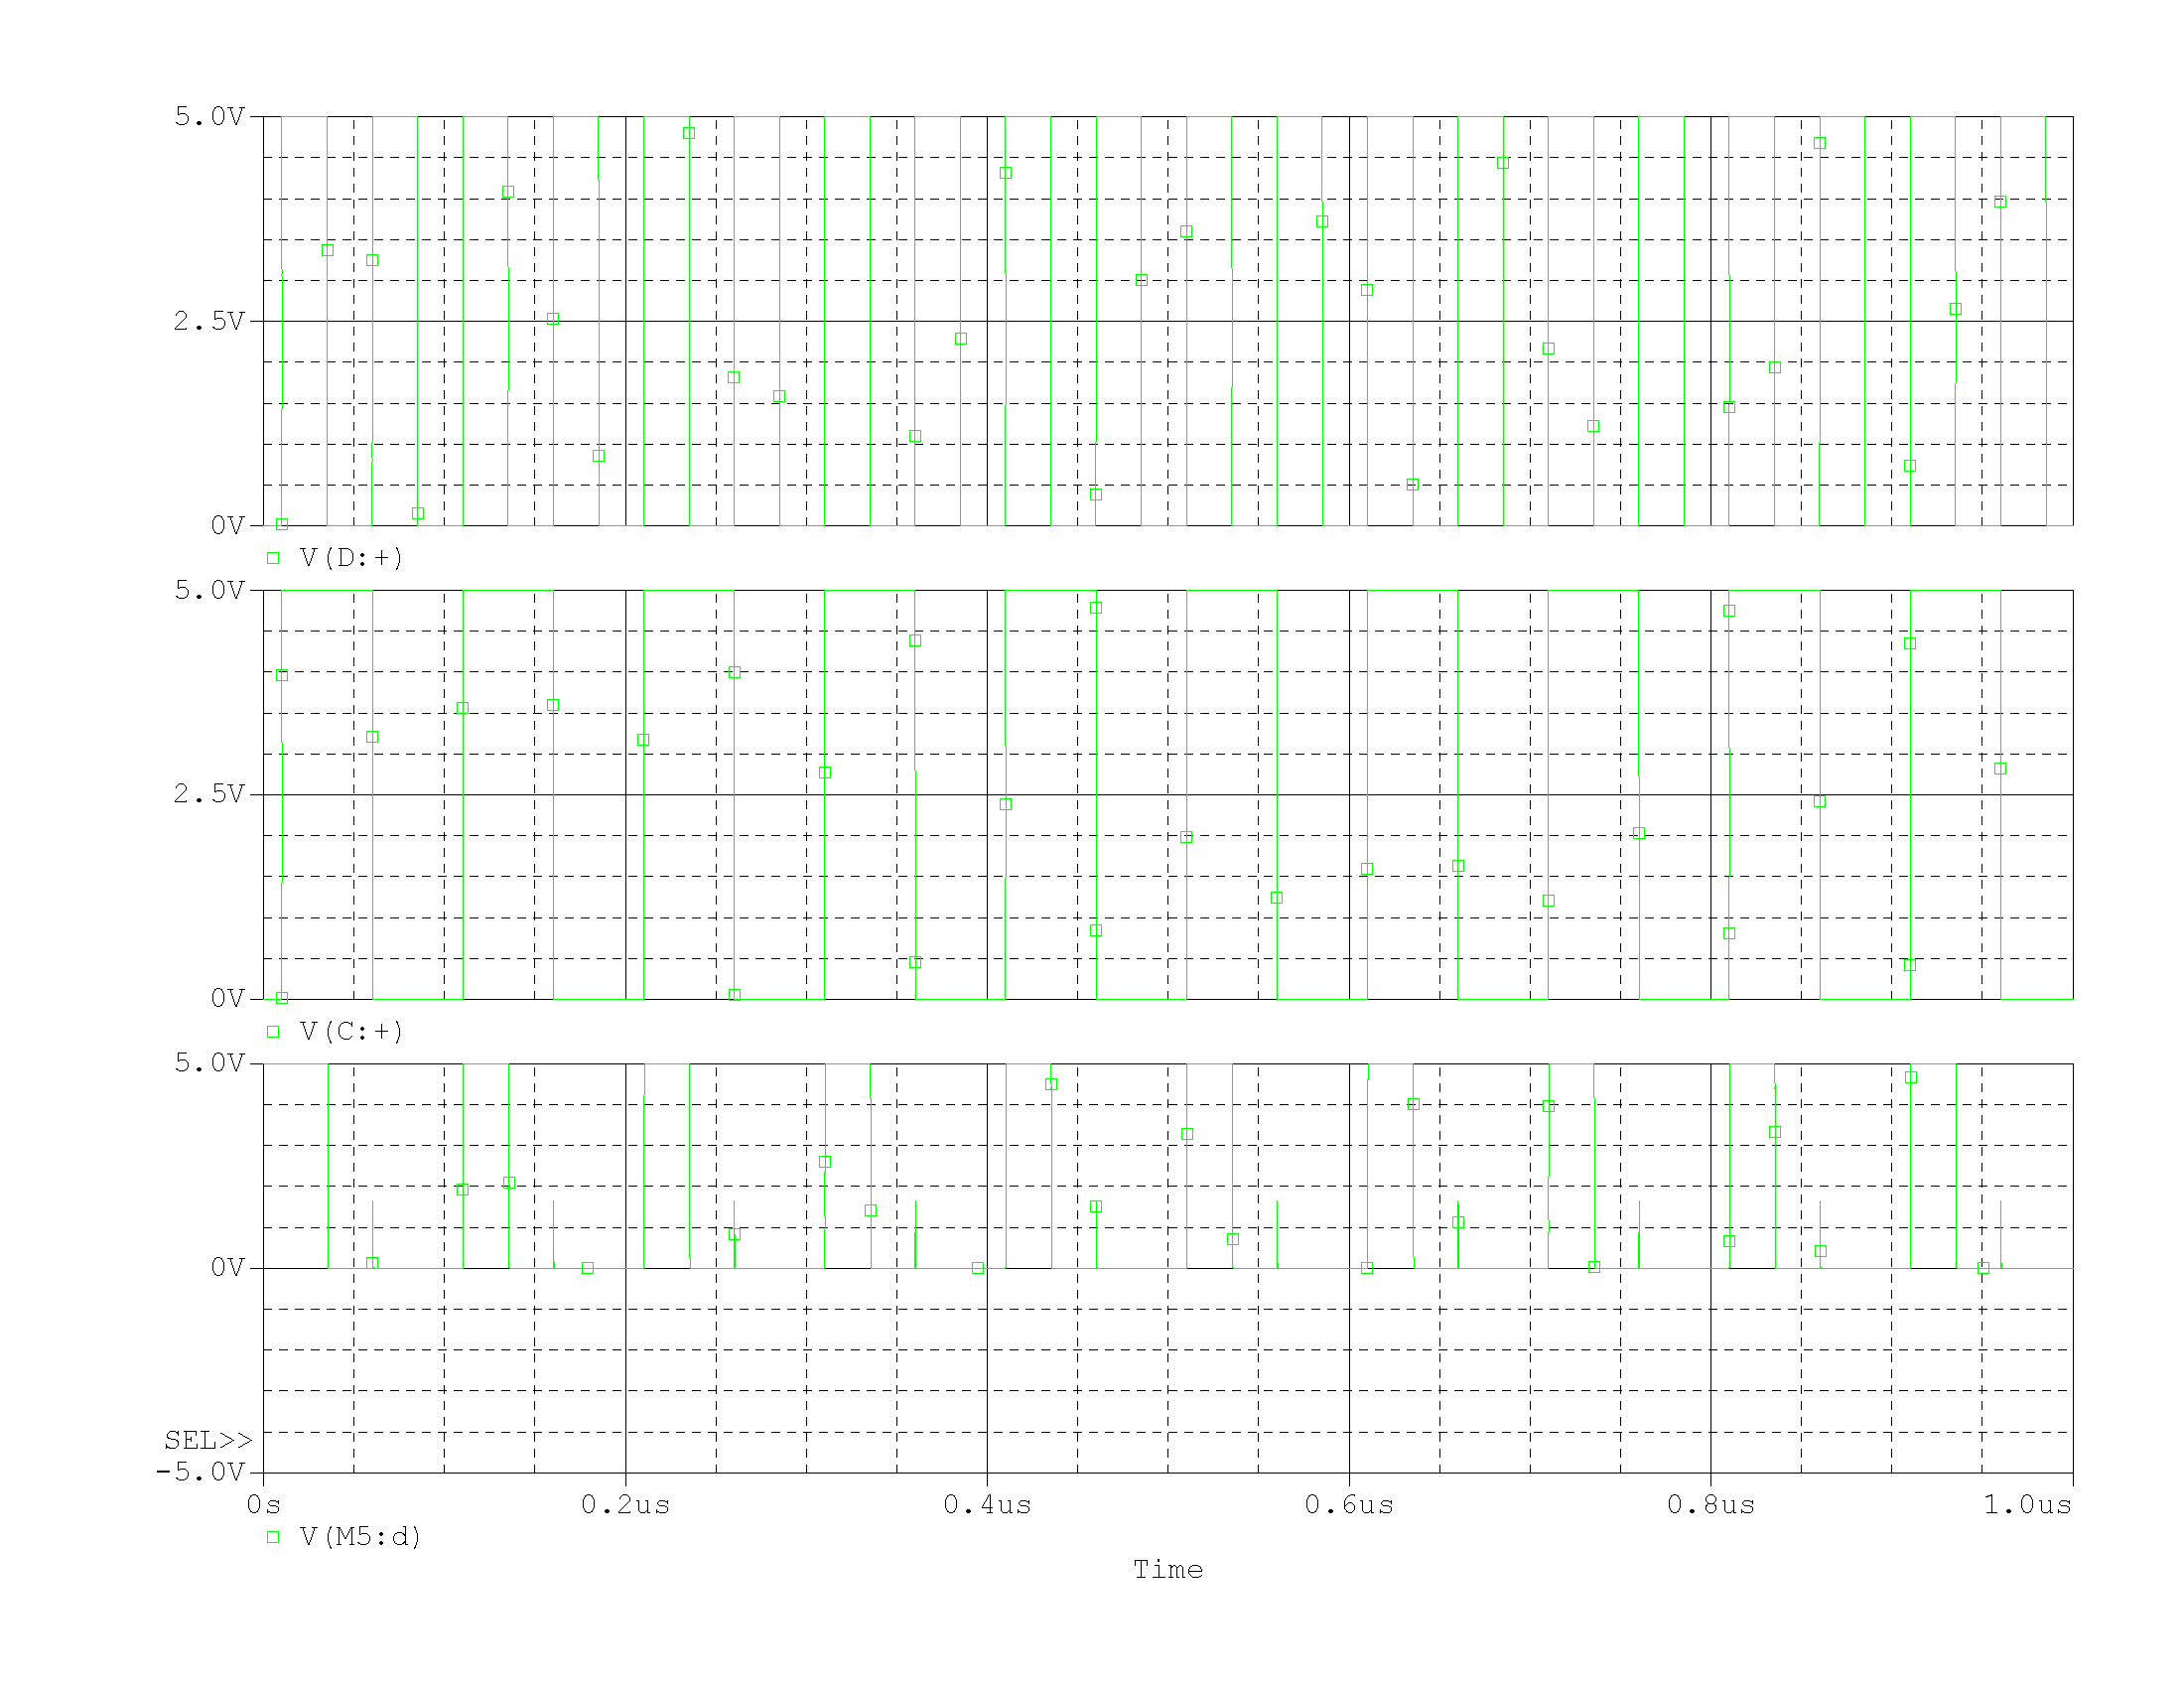
\includegraphics[width=1\linewidth]{./images/spec_sim}
	\caption{Simulation Results of D-Latch Using Inputs from Figure (\ref{fig:supplys})}
	\label{fig:spec_sim}
\end{figure}

\FloatBarrier
